\documentclass[8pt]{beamer}

\newif\ifplacelogo % create a new conditional
\placelogotrue % set it to true

\usetheme{Warsaw}
\usecolortheme{rose}
\usepackage{multicol}
\usepackage{epstopdf}
\usepackage[italic]{hepnames}
\usepackage{tikz}
\usepackage{listings}
\usepackage{times}
\usepackage{amsmath}
\usepackage{verbatim}
\usepackage{hyperref}
\usepackage{bbding}
\usepackage{gensymb}
\usepackage{upgreek}
\lstset{breakatwhitespace,
language=C++,
columns=fullflexible,
keepspaces,
breaklines,
tabsize=3, 
showstringspaces=false,
extendedchars=true}

% TikZ includes!!!
\usepackage{tikz}
\usetikzlibrary{backgrounds}
\usetikzlibrary{calc}
\tikzstyle{every picture}+=[remember picture]
\input{/home/oviazlo/Desktop/beamerPresentations/myReports/latexHelpScripts/tikzGrid.tex}


\begin{document}

% custom colors
\definecolor{olive}{rgb}{0.3, 0.4, .1}
\definecolor{fore}{RGB}{249,242,215}
\definecolor{back}{RGB}{51,51,51}
\definecolor{title}{RGB}{255,0,90}
\definecolor{dgreen}{rgb}{0.,0.6,0.}
\definecolor{gold}{rgb}{1.,0.84,0.}
\definecolor{JungleGreen}{cmyk}{0.99,0,0.52,0}
\definecolor{BlueGreen}{cmyk}{0.85,0,0.33,0}
\definecolor{RawSienna}{cmyk}{0,0.72,1,0.45}
\definecolor{Magenta}{cmyk}{0,1,0,0}

\definecolor{PixelColor}{RGB}{207,232,139}
\definecolor{SCTColor}{RGB}{167,166,255}
\definecolor{TRTColor}{RGB}{250,224,140}
\definecolor{grayColor}{RGB}{153,153,153}

\newcommand{\yRefPosOne}{0.0}
\newcommand{\xRefPosOne}{0.0}
\newcommand{\yRefPosTwo}{0.0}
\newcommand{\xRefPosTwo}{0.0}
\newcommand{\yRefIncrementOne}{0.0}
\newcommand{\xRefIncrementOne}{0.0}
\newcommand{\yRefIncrementTwo}{0.0}
\newcommand{\xRefIncrementTwo}{0.0}

\graphicspath{ {/home/oviazlo/Desktop/beamerPresentations/FCCee/pictures/CALOR2018/} }


\DeclareGraphicsExtensions{.eps, .pdf, .png}

\newcommand{\myBox}[2][pink] {
    \noindent\colorbox{#1}{
	\textbf{#2}
    }\par
}

% For nice block (provided by Oleh)
\tikzstyle{myBox} = [draw=red, fill=blue!1, very thick,
    rectangle, rounded corners, inner sep=5pt, inner ysep=9pt]
    
\tikzstyle{PixelBox} = [draw=PixelColor, fill=blue!1, very thick,
    rectangle, rounded corners, inner sep=5pt, inner ysep=9pt]
\tikzstyle{SCTBox} = [draw=SCTColor, fill=blue!1, very thick,
    rectangle, rounded corners, inner sep=5pt, inner ysep=9pt]
\tikzstyle{TRTBox} = [draw=TRTColor, fill=blue!1, very thick,
    rectangle, rounded corners, inner sep=5pt, inner ysep=9pt]

% poster advertisement
\newcommand{\myCenterBox}[2][pink] {
   {\centering
    \noindent\colorbox{#1}{
	\textbf{#2}
    }\par
  }
}

\newcommand{\mySmallCenterBox}[2][pink] {
   {\centering
    \noindent\colorbox{#1}{
	\textbf{{\small #2}}
    }\par
  }
}

\newcommand{\myVerySmallCenterBox}[2][pink] {
   {\centering
    \noindent\colorbox{#1}{
	\textbf{{\scriptsize #2}}
    }\par
  }
}

\newcommand{\backupbegin}{
   \newcounter{finalframe}
   \setcounter{finalframe}{\value{framenumber}}
}
\newcommand{\backupend}{
   \setcounter{framenumber}{\value{finalframe}}
}

\newcommand{\myNode}{\tikz[baseline,inner sep=1pt] \node[anchor=base]}

\tikzstyle{fancytitle} =[fill=white!15, text=black]

\definecolor{light-gray}{gray}{0.95}
% poster advertisement


\title[Calorimetry performance with CLD \hspace{14.0em}\insertframenumber/
\inserttotalframenumber]{ Calorimetry performance with CLD }


	\author[Oleksandr Viazlo]{Oleksandr Viazlo\\ 
	{\small on behalf of the CLICdp and FCC-ee collaborations}
	}
	\institute{\small CERN\\} 
	
       
	\date{22 May 2018}

% 	\logo{ \ifplacelogo \includegraphics[height=1.8cm]{./ID_week2/lund_uni-logo_s.pdf} \hspace{0.4cm} \fi}

	
%    	\frame{\titlepage}

   	

\placelogofalse




%*****************************************************************************
\begin{frame}{\large \large Single particle identification efficiency}
\renewcommand{\yRefPosOne}{-0.9}
\renewcommand{\xRefPosOne}{4.2}
\renewcommand{\xRefIncrementOne}{7.5}
\begin{tikzpicture}[overlay]

 \node[inner sep=0pt] (tmp) at (\xRefPosOne-1.7,\yRefPosOne-0.1)
%   {\includegraphics[width=6cm]{singleParticleEff/CLD_muon_eff.pdf}};
  {\includegraphics[width=6cm]{../may30_2018/PionMisreconstructedAsMuon.png}};
  
 \node[inner sep=0pt] (tmp) at (\xRefPosOne+4.5,\yRefPosOne-0.1)
%   {\includegraphics[width=6cm]{singleParticleEff/CLD_pion_eff.pdf}};
  {\includegraphics[width=6cm]{../may30_2018/may30_pions_eff.pdf}};


 \node  at (\xRefPosOne+1,\yRefPosOne+3.5) (box){%
    \begin{minipage}{1.1\textwidth}
  \begin{itemize}
   \item Muon identification algorithm: fit a track from hits in muon chambers $\to$ match muon chamber track with track from tracking system $\to$ identify hits from calorimeter which belong to muon track
%    \item Reconstruction parameters: muon track fit in yoke, track mathing, identification of muon hits in calorimeter
    \end{itemize}
    \end{minipage}
  };



  
%          \node  at (\xRefPosOne-3.1,\yRefPosOne+1.75) (box){%
%     \myCenterBox{\small Muons}
%     };     

       \node  at (\xRefPosOne+3,\yRefPosOne+2.25) (box){%
    \myCenterBox{\small Pions}
    };     


    
 \node  at (\xRefPosOne+1,\yRefPosOne-3.5) (box){%
    \begin{minipage}{\textwidth}
      \begin{itemize}
        \item First attempt to recover pion inefficiency: more strict requirement on track matching (Distance of closest approach 200mm $\to$ 80mm)
      \end{itemize}
    \end{minipage}
  };
 
 \end{tikzpicture}
\end{frame}
%*****************************************************************************
%*****************************************************************************
\begin{frame}{\large \large Single particle identification efficiency}
\renewcommand{\yRefPosOne}{-0.9}
\renewcommand{\xRefPosOne}{4.2}
\renewcommand{\xRefIncrementOne}{7.5}
\begin{tikzpicture}[overlay]

 \node[inner sep=0pt] (tmp) at (\xRefPosOne-1.7,\yRefPosOne+0.3)
%   {\includegraphics[width=6cm]{singleParticleEff/CLD_muon_eff.pdf}};
  {\includegraphics[width=6cm]{../may30_2018/table_muonReco.png}};
  
 \node  at (\xRefPosOne+4,\yRefPosOne+2.2) (box){%
    \begin{minipage}{0.5\textwidth}
      \begin{itemize}
        \item First six parameters - clustering of the hits in the muon system \\[0.2cm]
        \item The next three - to define the muon system cluster candidate \\[0.2cm]
        \item The next three - to match ID track to straight line fit of muon system hits \\[0.2cm]
        \item The final six - to acossiated Calo hits to the muon PFO \\[0.2cm]
      \end{itemize}
    \end{minipage}
  };

   \node[inner sep=0pt] (tmp) at (\xRefPosOne+4.5,\yRefPosOne-2.1)
%   {\includegraphics[width=6cm]{singleParticleEff/CLD_pion_eff.pdf}};
  {\includegraphics[width=5.5cm]{../may30_2018/may30_pions_eff_max_15_hits.png}};

 
 \end{tikzpicture}
\end{frame}
%*****************************************************************************
%*****************************************************************************
\begin{frame}{\large \large Single particle identification efficiency}
\renewcommand{\yRefPosOne}{-0.9}
\renewcommand{\xRefPosOne}{4.2}
\renewcommand{\xRefIncrementOne}{7.5}
\begin{tikzpicture}[overlay]

 \node[inner sep=0pt] (tmp) at (\xRefPosOne-1.7,\yRefPosOne-0.1)
%   {\includegraphics[width=6cm]{singleParticleEff/CLD_muon_eff.pdf}};
  {\includegraphics[width=6cm]{../may30_2018/xt90.pdf}};
  
 \node[inner sep=0pt] (tmp) at (\xRefPosOne+4.5,\yRefPosOne-0.1)
%   {\includegraphics[width=6cm]{singleParticleEff/CLD_pion_eff.pdf}};
  {\includegraphics[width=6cm]{../may30_2018/RhitMean.pdf}};


 \node  at (\xRefPosOne+1,\yRefPosOne+3.5) (box){%
    \begin{minipage}{1.1\textwidth}
  \begin{itemize}
   \item Look on cluster shape parameters of muon candidates
    \end{itemize}
    \end{minipage}
  };

    
%  \node  at (\xRefPosOne+1,\yRefPosOne-3.5) (box){%
%     \begin{minipage}{\textwidth}
%       \begin{itemize}
%         \item No 
%       \end{itemize}
%     \end{minipage}
%   };
 
 \end{tikzpicture}
\end{frame}
%*****************************************************************************


\backupbegin
%*****************************************************************************
\begin{frame}
\frametitle{BACKUP} 
 
\end{frame}
%*****************************************************************************
%*****************************************************************************
\begin{frame}{\large \large Single particle identification efficiency}
\renewcommand{\yRefPosOne}{-0.9}
\renewcommand{\xRefPosOne}{4.2}
\renewcommand{\xRefIncrementOne}{7.5}
\begin{tikzpicture}[overlay]

 \node[inner sep=0pt] (tmp) at (\xRefPosOne-1.7,\yRefPosOne-0.6)
%   {\includegraphics[width=6cm]{singleParticleEff/CLD_muon_eff.pdf}};
  {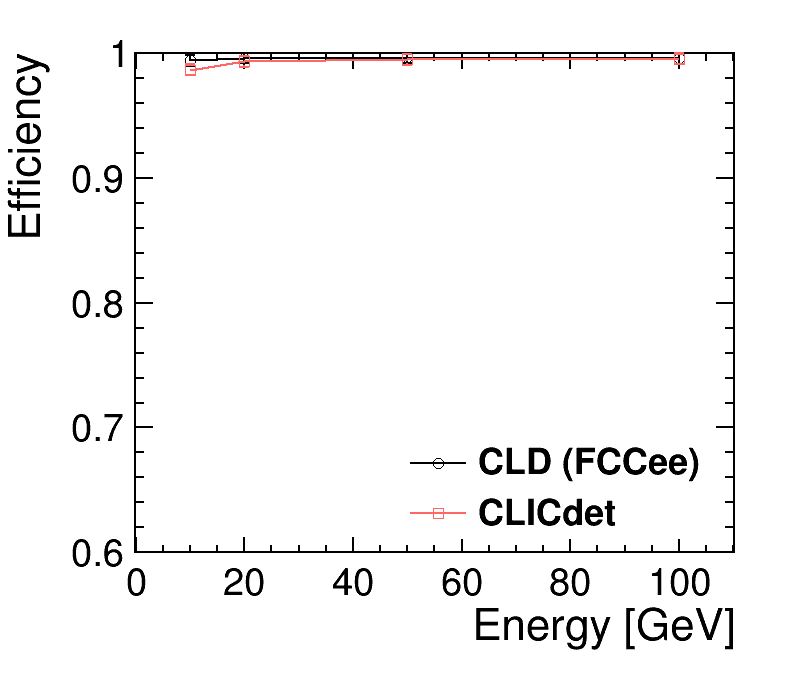
\includegraphics[width=6cm]{may21_muons_eff.pdf}};
  
 \node[inner sep=0pt] (tmp) at (\xRefPosOne+4.5,\yRefPosOne-0.6)
%   {\includegraphics[width=6cm]{singleParticleEff/CLD_pion_eff.pdf}};
  {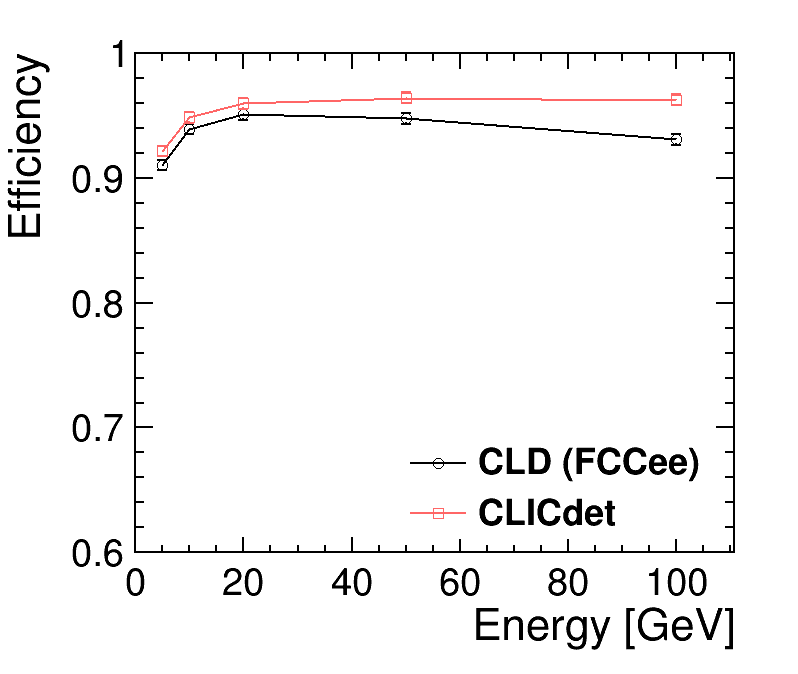
\includegraphics[width=6cm]{may21_pions_eff.pdf}};


 \node  at (\xRefPosOne+1,\yRefPosOne+3.3) (box){%
    \begin{minipage}{1.1\textwidth}
  \begin{itemize}

   \item Efficiency = fraction of matched reconstructed particles out of the simulated MC particles:
      \begin{itemize}
       \item reconstructed particle of the same type as simulated MC particle
       \item angular matching: $\Delta\theta <$ 1 mrad and $\Delta\phi <$ 2 mrad
       \item energy matching:\\
       - charged particles: $|p_T^{truth} - p_T^{PFO}| < 5\%$ $p_T^{truth} $ \\
       - photons: $\Delta$$E < 5\times\sigma$(ECal) $\approx 0.75\times \sqrt{E}$
      \end{itemize}
    \end{itemize}
    \end{minipage}
  };

  \node [TRTBox]  at (\xRefPosOne+4.8,\yRefPosOne+2.7) (box){%
  \begin{minipage}{0.4\textwidth}
   Sample: single particles with flat cos($\theta$) distribution and fixed energy
  \end{minipage}
  };


  
         \node  at (\xRefPosOne-3.1,\yRefPosOne+1.75) (box){%
    \myCenterBox{\small Muons}
    };     

       \node  at (\xRefPosOne+3,\yRefPosOne+1.75) (box){%
    \myCenterBox{\small Pions}
    };     

 \node[inner sep=0pt] (tmp) at (\xRefPosOne-0.1,\yRefPosOne+1.75)
  {\tiny WORK IN PROGRESS};
 
 \node[inner sep=0pt] (tmp) at (\xRefPosOne+6.1,\yRefPosOne+1.75)
  {\tiny WORK IN PROGRESS};
    
 \node  at (\xRefPosOne+1,\yRefPosOne-3.5) (box){%
    \begin{minipage}{\textwidth}
      \begin{itemize}
        \item $>$99$\%$ muon efficiency and 93-96$\%$ pion efficiency for E$>$10 GeV
        \item Inefficiency at high energies with CLD is caused by a larger rate of pions being mis-reconstructed as muons 
%         $\to$ optimization of muon requirements are needed
      \end{itemize}
    \end{minipage}
  };
 
 \end{tikzpicture}
\end{frame}
%*****************************************************************************
%*****************************************************************************
\begin{frame}{\large \large Pion identification efficiency (CLD)}
\renewcommand{\yRefPosOne}{-0.5}
\renewcommand{\xRefPosOne}{4.2}
\renewcommand{\xRefIncrementOne}{7.5}
\begin{tikzpicture}[overlay]

 \node[inner sep=0pt] (tmp) at (\xRefPosOne-1.7,\yRefPosOne-0.6)
  {\includegraphics[width=6cm]{../plots_FCCweek_workshop/singleParticleEff/pion_eff_vs_theta_E20.pdf}}; 
  
 \node[inner sep=0pt] (tmp) at (\xRefPosOne+4.5,\yRefPosOne-0.6)
  {\includegraphics[width=6cm]{../plots_FCCweek_workshop/singleParticleEff/pion_eff_vs_theta_E100.pdf}};


 \node  at (\xRefPosOne+1,\yRefPosOne+2.9) (box){%
    \begin{minipage}{1.1\textwidth}
  \begin{itemize}

   \item Pion ID efficiency and inefficiency as function of cos($\theta$)
    \end{itemize}
    \end{minipage}
  };


 \node  at (\xRefPosOne+1,\yRefPosOne-3.5) (box){%
    \begin{minipage}{\textwidth}
      \begin{itemize}
        \item High momentum pions more often are misreconstructed as muons in barrel
      \end{itemize}
    \end{minipage}
  };
   
       \node  at (\xRefPosOne-2.65,\yRefPosOne+1.75) (box){%
    \myCenterBox{\small 20 GeV pions}
    };     

       \node  at (\xRefPosOne+3.6,\yRefPosOne+1.75) (box){%
    \myCenterBox{\small 100 GeV pions}
    };     

%  \node[inner sep=0pt] (tmp) at (\xRefPosOne-0.1,\yRefPosOne+1.75)
%   {\tiny WORK IN PROGRESS};
%  
%  \node[inner sep=0pt] (tmp) at (\xRefPosOne+6.1,\yRefPosOne+1.75)
%   {\tiny WORK IN PROGRESS};
    
 \end{tikzpicture}
\end{frame}
%*****************************************************************************


\backupend
%********************************************************
\end{document}

